%Fiquemos com Deus e Nossa Senhora!
%Sao Jose de Cupertino rogai por nos que recorremos a vos!!!
%Honra teu Pai e tua Mãe!
% ### Uses XeLaTeX ### %
% ### Needs beamer-master ### %
\documentclass[aspectratio=169]{beamer} %. Aspect Ratio 16:9

\usetheme{AI2} % beamerthemeSprace.sty
\usepackage[portuguese]{babel}
\usepackage[utf8]{inputenc}
\usepackage[T1]{fontenc}
\usepackage{ragged2e,gensymb,bm,amsmath,amssymb}

\DeclareMathOperator*{\argmin}{arg\,min}
\DeclareMathOperator*{\argmax}{arg\,max}
\DeclareMathOperator{\sign}{sgn}

% DATA FOR FOOTER
\date{2021}
\title{- Kernel PCA}
\author{João Paulo Papa}
\institute{Advanced Institute for Artificial Intelligence (AI2)}

\begin{document}
% ####################################
% FIRST SLIDE 						:: \SliTit{This is the Title of the Talk}{A. B. Name}{Sprace}
% SUB-TITLE SLIDE 					:: \SliSubTit{<title>}{<explanation}
% SUB-SUB-TITLE SLIDE				:: \SliSubSubTit{<title>}{<explanation}
% SLIDE WITH TITLE 					:: \SliT{Title}{Content}
% SLIDE NO TITLE 						:: \Sli{Content} 
% SLIDE DOUBLE COLUMN WITH TITLE 	:: \SliDT{Title}{First Column}{Second Column}
% SLIDE DOUBLE COLUMN NO TITLE 		:: \SliD{First Column}{Second Column}
% SLIDE ADVANCED WITH TITLE 			:: \SliAdvT{Title}{Content}
% SLIDE ADVANCED NO TITLE 			:: \SliAdv{Content}
% SLIDE ADVANCED DOUBLE WITH TITLE 	:: \SliAdvDT{Title}{First Column}{Second Column}
% SLIDE ADVANCED DOUBLE NO TITLE 	:: \SliAdvD{First Column}{Second Column}
% SLIDE BLACK						:: \Black{ <Content> }
% SLIDE WHITE						:: \White{ <Content> }
% ITEMIZATION 						:: \begin{itemize}  \iOn{First} \iTw {Second} \iTh{Third} \end{itemize}
% COMMENT TEXT				 		:: \note{<comment>}
% SECTION 							:: \secx{Section} | \secxx{Sub-Section}
% BOLD SPRACE COLOR				:: \bfs{<text>}
% TABLE OF CONTENT					:: \tocitem{<title>}{<content>}
% LEFT ALIGN EQUATION				:: \begin{flalign*}  & <equation> &   \end{flalign*}
% CENTER ALIGN EQUATION	S			:: \begin{gather*} <equations>  \end{gather*}
% SLASH								:: \slashed{<>}
% BAR								:: \barr{<letter>} instead of \bar{<letter>}
% THEREFORE						:: use \portanto (larger and bold}
% 2 or 3 MATH SYMBOLS				:: \overset{<up>}{<down>} &  \underset{<below>}{\overset{<above>}{<middle>}}  
% INSERT TEXT IN FORMULA			:: \ins{<text>}
% EXERCISE							:: \exe{<exercise #>}{<exercise text>}
% SUGGESTED READING BOX			:: \sug{<references>}
% CITATION							:: \cittex{<citation>}
% CITATION DOUBLE COLUMN 			:: \cittexD{<citation>}
% TEXT POSITION						:: \texpos{<Xcm>}{<Ycm>}{<text>} origin = center of slide : x right | y down
% REFERENCE AT BOTTOM  S/D SLIDE		:: \refbotS{<reference>} \refbotD{<reference>}
% HIDDEN SLIDE						:: \hid
% COLOR BOX 						:: \blu{blue} + \red{rec} + \yel{yellow} + \gre{green} + \bege{beige}
% FRAME 							:: \fra{sprace} \frab{blue} \frar{red} + \fray{yellow} + \frag{green}		
% FIGURE 							:: \img{X}{Y}{<scale>}{Figure.png} 
% FIGURE							:: \includegraphics[scale=<scale>]{Figures/.png}
% FIGURE DOUBLE SLIDE NO TITLE		::  \img{-4}{0.5}{<scale>}{Figure.png} % Image 1st half
%									::  \img{4}{0.5}{<scale>}{Figure.png} % Image 2nd half
% FIGURE DOUBLE SLIDE WITH TITLE		::  \img{-4}{0}{<scale>}{Figure.png} % Image 1st half
%									::  \img{4}{0}{<scale>}{Figure.png} % Image 2nd half
% INCLUDING SWF (Flash)				:: \usepackage{media9} and \includemedia >> USE ACROBAT <<
%%%%%%%%%%%%%%%%%%%%%%%%%%%%%%%%%%%%%%%%%%%%%%%%%%
% ###############################################################################
% FIRST SLIDE
\SliTit{{\LARGE Kernel PCA}}{Advanced Institute for Artificial Intelligence -- AI2}{https://advancedinstitute.ai}
%%%%%%%%%%%%%%%%%%%%%%%%%%%%%%%%%%%%%%%%%%%%%%%%%%
% ###############################################################################
% SLIDE SUB-TITLE
%\SliSubTit{Sub-Title}{Description}{}
%%%%%%%%%%%%%%%%%%%%%%%%%%%%%%%%%%%%%%%%%%%%%%%%%%
% ###############################################################################
%\SliSubSubTit{Sub-Sub-Title}{Description}
 %%%%%%%%%%%%%%%%%%%%%%%%%%%%%%%%%%%%%%%%%%%%%%%%%%


\SliT{Introdução}{

\justifying \emph{Kernel PCA} (KPCA) é uma técnica que busca generalizar PCA visando realizar \textbf{redução não linear de dimensionalidade}. Lembrando que PCA assume que os dados estão em um espaço Euclidiano, ou seja, linear. Na hipótese que os dados estão em um espaço não linear, PCA não consegue garantir a sua otimalidade.\newline

\justifying Seja, então, um conjunto de dados ${\cal X}=\{\bm{x}_1,\bm{x}_2,\ldots,\bm{x}_m\}$ tal que $\bm{x}_i\in\mathbb{R}^n$ representa uma amostra no espaço de características original. A ideia do KPCA é fazer uso de uma função de mapeamento não linear, também conhecida por \emph{kernel}, $\phi(\bm{x})\in\mathbb{R}^{n^{\prime}}$, tal que $n^\prime>n$, visando mapear os dados para um espaço de maior dimensão. Geralmente, esses mapeamentos são custosos pois envolvem a projeção das amostras nestes espaços com maior dimensão. No entanto, podemos contornar isso com o \emph{kernel trick}, em que podemos \textbf{calcular o produto interno} no espaço de alta dimensão \textbf{sem a necessidade} de projeção dos dados.
}

\Sli{
\justifying Desta forma, KPCA realiza um aumento temporário da dimensionalidade do espaço para depois realizar a sua redução. \textbf{A ideia é incorporar não linearidades durante o processo de redução de dimensionalidade.}\newline

\justifying A primeira hipótese do KPCA é assumir que a média amostral após o mapeamento para o espaço de maior dimensão vale zero, ou seja:

\begin{equation}
	\bm{\mu}^\prime = \frac{1}{m}\sum_{i=1}^m\phi(\bm{x}_i) = 0,
\end{equation}
em que $\bm{\mu}^\prime\in\mathbb{R}^{n^{\prime}}$. Neste caso, KPCA assume que a média amostral está situada na origem do espaço de dados.
}

\Sli{
\justifying Já a matriz de covariância $\bm{\Sigma}^\prime\in\mathbb{R}^{n^\prime\times n^\prime}$ é dada por:

\begin{equation}
	\bm{\Sigma}^\prime = \frac{1}{m}\sum_{i=1}^m(\phi(\bm{x}_i)-\cancelto{0}{\bm{\mu}^\prime})(\phi(\bm{x}_i)-\cancelto{0}{\bm{\mu}^\prime})^T = \frac{1}{m}\sum_{i=1}^m\phi(\bm{x}_i)\phi(\bm{x}_i)^T.
\end{equation}
\justifying Temos que os autovetores $\bm{v}_k$ da matriz $\bm{\Sigma}$ são dados por:

\begin{equation}
	\bm{\Sigma}^\prime\bm{v}_k = \lambda\bm{v}_k,\ \ \forall k = 1,2,\ldots,n^\prime.
\end{equation}
}

\Sli{
\justifying Existe um teorema bastante importante que nos diz que os autovetores de $\bm{\Sigma}$ podem ser escritos como uma combinação linear das características, ou seja:

\begin{equation}
	\bm{v}_k = \sum_{i=1}^{m}\alpha_{ki}\phi(\bm{x}_i).
\end{equation}
Assim sendo, para calcularmos os autovetores da matriz de covariância $\bm{\Sigma}^\prime$, basta sabermos os vetores $\bm{\alpha}_k$. Substituindo-se a Equação 2 na Equação 3, temos que:

\begin{equation}
	\bm{\Sigma}^\prime\bm{v}_k = \underbrace{\frac{1}{m}\sum_{i=1}^m\phi(\bm{x}_i)\phi(\bm{x}_i)^T}_{\bm{\Sigma}^\prime}\bm{v}_k = \lambda\bm{v}_k. 
\end{equation}
}

\Sli{
\justifying A Equação 5 implica em:

\begin{equation}
	\bm{v}_k = \frac{1}{m\lambda}\sum_{i=1}^m\phi(\bm{x}_i)\phi(\bm{x}_i)^T\bm{v}_k = \frac{1}{m\lambda}\sum_{i=1}^m[\phi(\bm{x}_i)^T\bm{v}_k]\phi(\bm{x}_i) = \sum_{i=1}^{m}\alpha_{ki}\phi(\bm{x}_i),
\end{equation}
em que $\alpha_{ki} = \frac{1}{m\lambda}\phi(\bm{x}_i)^T\bm{v}_k$. Agora, substituindo-se a Equação 6 na Equação 5, temos que:

\begin{equation}
	\frac{1}{m}\sum_{i=1}^m\phi(\bm{x}_i)\phi(\bm{x}_i)^T\left(\sum_{j=1}^{m}\alpha_{ki}\phi(\bm{x}_i)\right) = \lambda\sum_{j=1}^{m}\alpha_{kj}\phi(\bm{x}_j).
\end{equation}
}

\Sli{
\justifying Reescrevendo a Equação 7, temos que:

\begin{equation}
	\frac{1}{m}\sum_{i=1}^m\phi(\bm{x}_i)\left(\sum_{j=1}^{m}\alpha_{kj}\phi(\bm{x}_i)^T\phi(\bm{x}_j)\right) = \lambda\sum_{j=1}^{m}\alpha_{kj}\phi(\bm{x}_j).
\end{equation}
Fazendo uso do \emph{kernel trick}, ou seja, $K(\bm{x}_i,\bm{x}_j)=\phi(\bm{x}_i)^T\phi(\bm{x}_j)$ temos que:

\begin{equation}
	\frac{1}{m}\sum_{i=1}^m\phi(\bm{x}_i)\left(\sum_{j=1}^{m}\alpha_{kj}K(\bm{x}_i,\bm{x}_j)\right) = \lambda\sum_{j=1}^{m}\alpha_{kj}\phi(\bm{x}_j).
\end{equation}
}

\Sli{
\justifying Multiplicando ambos lados da Equação 9 por $\phi(\bm{x}_l)^T$, temos que:

\begin{equation}
	\frac{1}{m}\sum_{i=1}^m\phi(\bm{x}_l)^T\phi(\bm{x}_i)\left(\sum_{j=1}^{m}\alpha_{kj}K(\bm{x}_i,\bm{x}_j)\right) = \lambda\sum_{j=1}^{m}\alpha_{kj}\phi(\bm{x}_l)^T\phi(\bm{x}_j).
\end{equation}
Usando novamente o \emph{kernel trick}, temos que:

\begin{equation}
	\frac{1}{m}\sum_{i=1}^mK(\bm{x}_l,\bm{x}_i)\left(\sum_{j=1}^{m}\alpha_{kj}K(\bm{x}_i,\bm{x}_j)\right) = \lambda\sum_{j=1}^{m}\alpha_{kj}K(\bm{x}_l,\bm{x}_i).
\end{equation}
Temos que nossa formulação está, agora, escrita em função da matriz de \emph{kernel}.
}

\Sli{
\justifying Podemos expressar a Equação 11 em sua notação matriz-vetor, como segue:

\begin{equation}
	\bm{K}^2\bm{\alpha}_k = (\lambda m)\bm{K}\bm{\alpha}_k.
\end{equation}
Multiplicando-se ambos lados por $\bm{K}^{-1}$, temos que:

\begin{equation}
	\bm{K}\bm{\alpha}_k = (\lambda m)\bm{\alpha}_k.
\end{equation}
Quem são os $\bm{\alpha}_k$? São os \textbf{autovetores} da matriz de \emph{kernel}!
}

\Sli{
\justifying Para uma dada amostra $\bm{x}$, calculamos a sua projeção na $k$-ésima componente da seguinte forma:

\begin{equation}
	\hat{\bm{x}} = \phi(\bm{x})^T\bm{v}_k = \underbrace{\sum_{i=1}^n\alpha_{ki}\phi(\bm{x}_i)}_{\bm{v}_k}\phi(\bm{x})^T = \sum_{i=1}^n\alpha_{ki}K(\bm{x},\bm{x}_i).
\end{equation}
Basicamente, a projeção de uma amostra $\bm{x}$ na $k$-ésima componente resume-se a realizar o seu mapeamento para um espaço de maior dimensão com $\phi(\bm{x})$ e depois projetar em $\bm{v}_k$. \textbf{A vantagem do \emph{kernel trick} é que não precisamos calcular explicitamente $\phi(\bm{x}_i)$, $\forall i$, basta apenas computar a matriz de \emph{kernel} diretamente do conjunto de dados.}
}

\Sli{
\justifying Quais tipos de \emph{kernel} podemos utilizar? Os mais empregados são:

\begin{itemize}
	\item Polinomial: $K(\bm{x}_i,\bm{x}_j) = (\bm{x}_i^T\bm{x}_j+c)^d$, em que $c\geq0$ é uma constante e $d$ o grau do polinômio.
	\item Gaussiano (RBF): $K(\bm{x}_i,\bm{x}_j) = \exp\left\{-\frac{\norm{\bm{x}_i-\bm{x}_j}^2}{2\sigma^2}\right\}$.
\end{itemize}
Note, também, que se o dado projetado não tiver média nula, precisamos centralizá-lo da seguinte maneira:

\begin{equation}
	\tilde{\phi}(\bm{x}_i) = \phi(\bm{x}_i) - \frac{1}{m}\sum_{j=1}^m\phi(\bm{x}_j).
\end{equation}
}

\Sli{
\justifying Já a matriz \emph{kernel} correspondente (centralizada) é dada por:

\begin{align}\nonumber
\tilde{K}(\bm{x}_i,\bm{x}_j) &= \tilde{\phi}(\bm{x}_i)^T\tilde{\phi}(\bm{x}_j) = \left(\phi(\bm{x}_i)-\frac{1}{m}\sum_{k=1}^m\phi(\bm{x}_k)\right)^T\left(\phi(\bm{x}_j)-\frac{1}{m}\sum_{k=1}^m\phi(\bm{x}_k)\right)\\
\begin{split}
&=\phi(\bm{x}_i)^T\phi(\bm{x}_j)-\frac{1}{m}\sum_{k=1}^m\phi(\bm{x}_i)^T\phi(\bm{x}_k)-\frac{1}{m}\sum_{k=1}^m\phi(\bm{x}_k)^T\phi(\bm{x}_j)\\
	&\qquad +\frac{1}{m^2}\sum_{k=1}^m\sum_{l=1}^m\phi(\bm{x}_k)^T\phi(\bm{x}_l)
\end{split}\\
\begin{split}
&= K(\bm{x}_i,\bm{x}_j)-\frac{1}{m}\sum_{k=1}^mK(\bm{x}_i,\bm{x}_j)-\frac{1}{m}\sum_{k=1}^mK(\bm{x}_k,\bm{x}_j)\\
&\qquad+\frac{1}{n^2}\sum_{k=1}^m\sum_{l=1}^mK(\bm{x}_k,\bm{x}_l).
\end{split}\nonumber
\end{align}
}

\Sli{
Em sua forma matricial, podemos escrever a Equação 16 como segue (matriz Gram):

\begin{equation}
	\tilde{\bm{K}} = \bm{K}-1_m\bm{K}-\bm{K}1_m+1_m\bm{K}1_m,
\end{equation}
em que $1_n\in\mathbb{R}^{m\times m}$ é uma matriz com todos elementos iguais à $1/m$. Vejamos, agora, o algoritmo do KPCA:

\begin{enumerate}
	\item Construir matriz \emph{kernel} $\bm{K}$ a partir dos dados, em que $K_{i,j} = K(\bm{x}_i,\bm{x}_j)$.
	\item Construir matriz Gram $\tilde{\bm{K}}$ utilizando a Equação 17.
	\item Utilize Equação 13 para encontrar os autovetores $\bm{\alpha}_k$ (use $\tilde{\bm{K}}$).
	\item Calcule os $d$ componentes principais utilizando a Equação 14.
\end{enumerate}
}

\Sli{
\justifying Exemplos de projeções utilizando PCA e KPCA.

\begin{center}
\begin{tabular}{cc}
	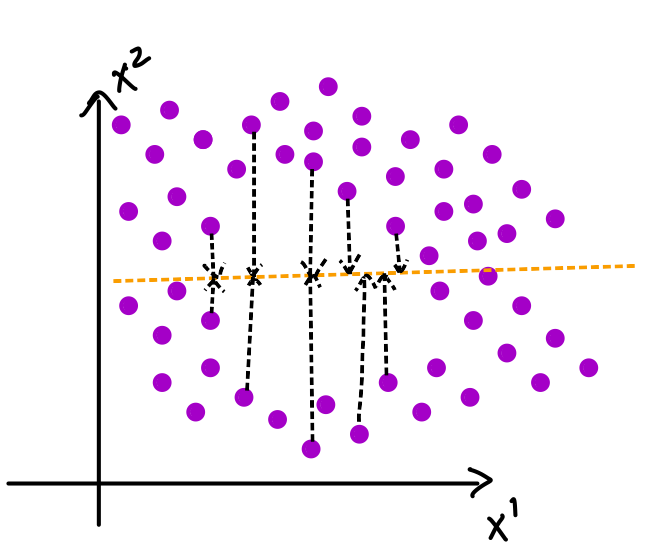
\includegraphics[scale=0.19]{./figs/KPCA_Fig1.png} &\hspace{2cm}
	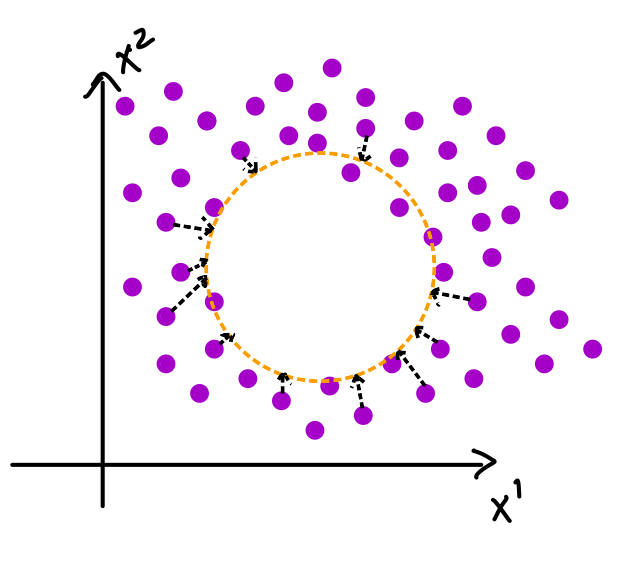
\includegraphics[scale=0.19]{./figs/KPCA_Fig2.png} \\
	PCA & \hspace{2cm}KPCA
\end{tabular}
\end{center}
}

\Sli{
\justifying Um agradecimento especial ao \textbf{Prof. Alexandre Levada} do Centro de Ciências Exatas e de Tecnologia, Departamento de Computação, Universidade Federal de São Carlos, pelas notas de aula.
}

\end{document}